\documentclass[10pt]{article}


\title{Transformers as Decision Makers: Provable In-Context Reinforcement Learning via Supervised Pretraining}

\date{\today}
\author{
  Licong Lin\thanks{UC Berkeley. Email: \texttt{liconglin@berkeley.edu}}\hspace{.35em}
  \and
  Yu Bai\thanks{Salesforce AI Research. Email: \texttt{yu.bai@salesforce.com}}\hspace{.35em}\footnotemark[4]
  \and
  Song Mei\thanks{UC Berkeley. Email: \texttt{songmei@berkeley.edu}}\hspace{.35em}\thanks{Equal contribution.}
}

\def\shownotes{0}  %
\ifnum\shownotes=1
\newcommand{\authnote}[2]{{\scriptsize $\ll$\textsf{#1 notes: #2}$\gg$}}
\else
\newcommand{\authnote}[2]{}
\fi
\newcommand{\yub}[1]{{\color{red}\authnote{Yu}{#1}}}
\newcommand{\cfn}[1]
{{\color{blue}\authnote{Song}{#1}}}
\newcommand{\lc}[1]{{\color{blue}\authnote{Licong}{#1}}}
\newcommand{\todo}[1]{{\color{blue}$\ll$\textsf{\footnotesize TODO:
      {#1}$\gg$}}}

\makeatletter
\def\blfootnote{\gdef\@thefnmark{}\@footnotetext}
\makeatother

\begin{document}

\maketitle


\begin{abstract}



Large transformer models pretrained on offline reinforcement learning datasets have demonstrated remarkable in-context reinforcement learning (ICRL) capabilities, where they can make good decisions when prompted with interaction trajectories from unseen environments. However, when and how transformers can be trained to perform ICRL have not been theoretically well-understood. In particular, it is unclear which reinforcement-learning algorithms transformers can perform in context, and how distribution mismatch in offline training data affects the learned algorithms.
This paper provides a theoretical framework that analyzes supervised pretraining for ICRL. This includes two recently proposed training methods --- algorithm distillation and decision-pretrained transformers. First, assuming model realizability, we prove the supervised-pretrained transformer will imitate the conditional expectation of the expert algorithm given the observed trajectory. The generalization error will scale with model capacity and a distribution divergence factor between the expert and offline algorithms. Second, we show transformers with ReLU attention can efficiently approximate near-optimal online reinforcement learning algorithms like LinUCB and Thompson sampling for stochastic linear bandits, and UCB-VI for tabular Markov decision processes. This provides the first quantitative analysis of the ICRL capabilities of transformers pretrained from offline trajectories.






\end{abstract}
\section{Introduction}


The transformer architecture~\citep{vaswani2017attention} for sequence modeling has become a key weapon for modern artificial intelligence, achieving success in language~\citep{devlin2018bert,brown2020language,openai2023gpt} and vision~\citep{dosovitskiy2020image}. Motivated by these advances, the research community has actively explored how to best harness transformers for reinforcement learning (RL)~\citep{chen2021decision, janner2021offline, lee2022multi, reed2022generalist, laskin2022context, lee2023supervised,yang2023foundation}. While promising empirical results have been demonstrated, the theoretical understanding of transformers for RL remains limited. %



This paper provides theoretical insights into in-context reinforcement learning (ICRL)---an emerging approach that utilizes sequence-to-sequence models like transformers to perform reinforcement learning in newly encountered environments. In ICRL, the model takes as input the current state and past interaction history with the environment (the \emph{context}), and outputs an action. The key hypothesis in ICRL is that pretrained transformers can act as \emph{RL algorithms}, progressively improving their policy based on past observations. Approaches such as Algorithm Distillation \citep{laskin2022context} and Decision-Pretrained Transformers \citep{lee2023supervised} have demonstrated early successes, finding that \emph{supervised pretraining} can produce good ICRL performance. However, many concrete theoretical questions remain open about the ICRL capabilities of transformers, including but not limited to (1) what RL algorithms can transformers implement in-context; (2) what performance guarantees (e.g. regret bounds) can such transformers achieve when used iteratively as an online RL algorithm; and (3) when can supervised pretraining find such a good transformer. Specifically, this paper investigates the following open question:
\begin{center}
\emph{How can supervised pretraining on Transformers learn in-context reinforcement learning?}
\end{center}


In this paper, we initiate a theoretical study of the ICRL capability of transformers under supervised pretraining to address the open questions outlined above. We show that (1) Transformers can implement prevalent RL algorithms, including LinUCB and Thompson sampling for stochastic linear bandits, and UCB-VI for tabular Markov decision processes; (2) The algorithms learned by transformers achieve near-optimal regret bounds in their respective settings; (3) Supervised pretraining find such algorithms as long as the sample size scales with the covering number of transformer class and distribution ratio between expert and offline algorithms. %

\paragraph{Summary of contributions and paper outline}
\begin{itemize}[leftmargin=1.5em]
\item We propose a general framework for supervised pretraining approaches to meta-reinforcement learning (Section~\ref{sec:framework}). This framework encompasses existing methods like Algorithm Distillation \citep{laskin2022context}, where the expert and context algorithms are identical, as well as Decision-Pretrained Transformers \citep{lee2023supervised}, where the expert generates optimal actions for the MDP. It also includes approximate DPT variants where the expert estimates optimal actions from full interaction trajectories.
\item We prove that the supervised-pretrained transformer will imitate the conditional expectation of the expert algorithm given the observed trajectory (Section~\ref{sec:supervised-pretraining}). The generalization error scales with both model capacity and a distribution ratio measuring divergence between the expert algorithm and the algorithm that generated offline trajectories.

\item We demonstrate that transformers can effectively approximate several near-optimal reinforcement learning algorithms by taking observed trajectories as context inputs (Section~\ref{sec:ICRL}). Specifically, we show transformers can approximate LinUCB (Section~\ref{sec:LinUCB-statement}) and Thompson sampling algorithms (Section~\ref{sec:TS-statement}) for stochastic linear bandit problems, and UCB-VI (Section~\ref{sec:Tabular-MDP-statement}) for tabular Markov decision processes. Combined with the generalization error bound from supervised pretraining and regret bounds of these RL algorithms, this provides regret bounds for supervised-pretrained transformers.
\item Preliminary experiments validate that transformers can perform ICRL in our setup (Section~\ref{sec:experiments}).
\item Technically, we prove efficient approximation of LinUCB by showing transformers can implement accelerated gradient descent for solving ridge regression (\cref{sec:pf_thm:approx_smooth_linucb}), enabling fewer attention layers than the vanilla gradient descent approach in \cite{bai2023transformers}. To enable efficient Thompson sampling implementation, we prove transformers can compute matrix square roots through the Pade decomposition (\cref{sec:pf_thm:approx_thompson_linear-formal}). These approximation results are interesting in their own right.
\end{itemize}

\subsection{Related work}\label{sec:related-work}

\paragraph{Meta-learning and meta-reinforcement learning} In-context reinforcement learning can be cast into the framework of meta-learning and meta-reinforcement learning \citep{schmidhuber1987evolutionary, schmidhuber1992learning, bengio1990learning, naik1992meta, ishii2002control, schaul2010metalearning, thrun2012learning}. More recently, a line of work focuses on meta-learn certain shared structures such as the dynamics of the shared tasks \citep{fu2016one, nagabandi2018learning}, a task context identifier \citep{rakelly2019efficient, humplik2019meta, zintgraf2019varibad}, exploration strategies \citep{gupta2018meta}, or the initialization of the network policy \citep{finn2017model, hochreiter2001learning, nichol2018first, rothfuss2018promp}. Theories for this last approach of model-agnostic meta-learning have been explored by \cite{wang2020global}.

Our work focuses on a more agnostic approach to learning the learning algorithm itself \citep{wang2016learning, duan2016rl, dorfman2021offline, mitchell2021offline, li2020focal, pong2022offline, laskin2022context, lee2023supervised}. Among these works, \cite{wang2016learning, duan2016rl} focus on the online meta-RL setting with the training objective to be the total reward. Furthermore, \cite{dorfman2021offline, mitchell2021offline, li2020focal, pong2022offline} focus on offline meta-RL, but their training objectives differ from the cross entropy loss used here, requiring explicit handling of distribution shift. The supervised pretraining approach we consider is most similar to the algorithm distillation methods of \cite{laskin2022context} and the decision-pretrained transformers of \cite{lee2023supervised}. We provide quantitative sample complexity guarantees and transformer constructions absent from previous work.


\paragraph{In-context learning}

The in-context learning (ICL) capability of pretrained transformers has gained significant attention since being demonstrated on GPT-3 \cite{brown2020language}. Recent work investigates why and how pretrained transformers perform ICL \citep{garg2022can, li2023transformers, von2023transformers, akyurek2022learning, xie2021explanation, bai2023transformers,
zhang2023trained, ahn2023transformers, raventos2023pretraining}. In particular, \cite{xie2021explanation} propose a Bayesian framework explaining how ICL works. \cite{garg2022can} show transformers can be trained from scratch to perform ICL of simple function classes.  \cite{von2023transformers, akyurek2022learning, bai2023transformers} demonstrate transformers can implement in-context learning algorithms via in-context gradient descent, with \cite{bai2023transformers} showing transformers can perform in-context algorithm selection. \cite{zhang2023trained} studied training dynamics of a single attention layer for in-context learning of linear functions. Our work focuses on the related but distinct capability of in-context decision-making for pretrained transformers.

\paragraph{Transformers for decision making} Besides the ICRL approach, recent work has proposed goal-conditioned supervised learning (GCSL) for using transformers to make decisions \citep{chen2021decision, janner2021offline, lee2022multi, reed2022generalist, brohan2022rt, shafiullah2022behavior, yang2023foundation}. In particular, Decision Transformer (DT) \citep{chen2021decision, janner2021offline} uses transformers to autoregressively model action sequences from offline data, conditioned on the achieved return. During inference, one queries the model with a desired high return. Limitations and modifications of GCSL have been studied in \cite{yang2022dichotomy, paster2022you, vstrupl2022upside, brandfonbrener2022does}. A key distinction between GCSL and ICRL is that GCSL treats the transformer as a policy, whereas ICRL treats it as an algorithm for improving the policy based on observed trajectories.



\paragraph{Expressivity of transformers} The transformer architecture, introduced by \cite{vaswani2017attention}, has revolutionized natural language processing and is used in most recently developed large language models like BERT and GPT \citep{devlin2018bert, brown2020language}. The expressivity of transformers has been extensively studied~\citep{yun2019transformers, perez2019turing, hron2020infinite,yao2021self, bhattamishra2020computational, zhang2022unveiling, liu2022transformers, wei2022statistically, fu2023can, bai2023transformers, akyurek2022learning, von2023transformers}. Deep neural networks such as ResNets and transformers have been shown to efficiently approximate various algorithms, including automata \citep{liu2022transformers}, Turing machines \citep{wei2022statistically}, variational inference \citep{mei2023deep}, and gradient descent \citep{bai2023transformers, akyurek2022learning, von2023transformers}. Our work provides efficient transformer constructions that implement accelerated gradient descent and matrix square root algorithms, complementing existing expressivity results.





\paragraph{Statistical theories of imitation learning} Our generalization error analysis adapts classical analysis of maximum-likelihood estimator \citep{geer2000empirical}. The error compounding analysis for imitation learning appeared in early works \citep{ross2011reduction, ross2010efficient}. More recent theoretical analyses of imitation learning also appear in \cite{rajaraman2020toward, rajaraman2021provably, rashidinejad2021bridging}.



\section{Framework for In-Context Reinforcement Learning}\label{sec:framework}


Let $\cM$ be the space of decision-making environments, where each environment $\inst \in \cM$ shares the same number of rounds $\totlen$ and state-action-reward spaces $\{ \statesp_t,  \actionsp_t, \rewardsp_t \}_{t \in [\totlen]}$. Each $\inst = \{\transmodel_\inst^{t-1}, \rewmodel_\inst^t \}_{t \in [\totlen]}$ has its own transition model $\transmodel_\inst^t: \statesp_{t} \times \actionsp_{t} \to \Delta(\statesp_{t+1})$ (with $\statesp_0$, $\actionsp_0 = \{ \emptyset \}$ so $\transmodel_\inst^0(\cdot) \in \Delta(\statesp_1)$ gives the initial state distribution) and reward functions $\rewmodel_\inst^{t}: \statesp_{t} \times \actionsp_{t} \to \Delta(\rewardsp_t)$. We equip $\cM$ with a distribution $\prior \in \Delta(\cM)$, the environment prior. While this setting is general, we later give concrete examples taking $\cM$ as $\totlen$ rounds of bandits or $K$ episodes of $H$-step MDPs with $\totlen = K H$.

\paragraph{Distributions of offline trajectories} We denote a partial interaction trajectory, consisting of observed state-action-reward tuples, by $\dset_t=\{(\state_1,\action_1,\reward_1),\ldots,(\state_t,\action_t,\reward_t)\} \in \trajsp_t = \prod_{s \le t} (\statesp_s \times \actionsp_s \times \rewardsp_s)$ and write $\dset = \dset_{\totlen}$ for short. An algorithm $\sAlg$ maps a partial trajectory $\dset_{t-1} \in \trajsp_{t-1}$ and state $\state_t \in \statesp_t$ to a distribution over the actions $\sAlg(\cdot | \dset_{t-1}, \state_t) \in \Delta(\actionsp_t)$. Given an environment $\inst$ and algorithm $\sAlg$, the distribution over a full trajectory $\dset_\totlen$ is fully specified:
\begin{align*}
\textstyle \P_{\inst}^{\sAlg}(\dset_\totlen) =
\prod_{t=1}^{\totlen}\transmodel_{\inst}^{t-1}(\state_{t}|\state_{t-1},\action_{t-1}) \sAlg(\action_t|\dset_{t-1},\state_t)\rewmodel_{\inst}^t(\reward_t|\state_t,\action_t).
\end{align*}
In supervised pretraining, we use a \textit{context algorithm} $\sAlg_0$ (which we also refer to as the offline algorithm) to collect the offline trajectories $\dset_\totlen$. For each trajectory $\dset_\totlen$, we also assume access to expert actions $\eaction = ( \eaction_t \in \actionsp_t )_{t \in \totlen} \sim \sAlg_{\shortexp}(\cdot | \dset_\totlen, \inst)$, sampled from an expert algorithm $\sAlg_{\shortexp}: \trajsp_\totlen \times \inst \to \prod_{t \in [\totlen]} \Delta(\actionsp_t)$. This expert could omnisciently observe the full trajectory $\dset_\totlen$ and environment $\inst$ to recommend actions. Let $\adset_\totlen = \dset_\totlen \cup \{ \eaction \}$ be the augmented trajectory. Then we have
\begin{align*}
\textstyle \P^{\sAlg_0,\sAlg_{\shortexp}}_{\inst}(\adset_\totlen)=\P^{\sAlg_0}_{\inst}(\dset_\totlen)\prod_{t=1}^\totlen \sAlg_{\shortexp}^t (\eaction_t|\dset_{\totlen},\inst).
\end{align*}
We denote $\P^{\sAlg_0,\sAlg_\shortexp}_{\prior}$ as the joint distribution of $(\inst,\adset_\totlen)$ where $\inst \sim \prior$ and $\adset_\totlen \sim \P^{\sAlg_0,\sAlg_\shortexp}_{\inst}$, and $\P^{\sAlg_0}_{\prior}$ as the joint distribution of $(\inst,\dset_\totlen)$ where $\inst \sim \prior$ and $\dset_\totlen \sim \P^{\sAlg_0}_{\inst}$.

\paragraph{Three special cases of expert algorithms} We consider three special cases of the expert algorithm $\sAlg_{\shortexp}$, corresponding to three supervised pretraining setups:
\begin{itemize}[leftmargin=1.5em]
\item[(a)] {\it Algorithm distillation \citep{laskin2022context}. } The algorithm depends only on the partial trajectory $\dset_{t-1}$ and current state $\state_t$: $\sAlg_{\shortexp}^t(\cdot|\dset_{\totlen},\inst) = \sAlg_{\shortexp}^t(\cdot|\dset_{t-1},\state_t)$. For example, $\sAlg_{\shortexp}$ could be a bandit algorithm like the Uniform Confidence Bound (UCB).
\item[(b)] {\it Decision pretrained transformer (DPT) \citep{lee2023supervised}. } The algorithm depends on the environment $\inst$ and the current state $s_t$: $\sAlg_{\shortexp}^t(\cdot|\dset_\totlen, \inst) = \sAlg_{\shortexp}^t(\cdot|s_t, \inst)$. For example,  $\sAlg_{\shortexp}$ could output the optimal action $\action^*_t$ in state $\state_t$ for environment $\inst$.
\item[(c)]{\it Approximate DPT. } The algorithm depends on the full trajectory $\dset_{\totlen}$ but not the environment $\inst$: $\sAlg_{\shortexp}^t(\cdot|\dset_\totlen, \inst) =\sAlg_{\shortexp}^t(\cdot|\dset_\totlen)$. For example, $\sAlg_{\shortexp}$ could estimate the optimal action $\widehat \action^*_t$ from the entire trajectory $\dset_\totlen$.
\end{itemize}
For any expert algorithm $\sAlg_{\shortexp}$, we define its reduced algorithm where the $t$-th step is $$\osAlg_{\shortexp}(\cdot|\dset_{t-1},\state_t) := \E_\prior^{\sAlg_0}[\sAlg_{\shortexp}^t(\cdot|\dset_\totlen,\inst)|\dset_{t-1},\state_t].$$ The expectation on the right is over $\P_{\prior}^{\sAlg_0} ( \dset_\totlen, \inst |\dset_{t-1},\state_t) =\prior(\inst) \cdot \P_\inst^{\sAlg_0}(\dset_\totlen) / \P_\inst^{\sAlg_0}(\dset_{t-1},\state_t).$ Note that the reduced expert algorithm $\osAlg_{\shortexp}$ generally depends on the context algorithm $\sAlg_0$. However, for cases (a) and (b), $\osAlg_{\shortexp}$ is independent of the context algorithm $\sAlg_0$. Furthermore, in case (a), we have $\osAlg_{\shortexp}^t = \sAlg_{\shortexp}^t$.

\begin{comment}
\sm{I will start from here.}

\subsection{General framework}
Suppose the data collected for pretraining have the following form:
\begin{itemize}[leftmargin=1.5em]
\item   Sample a problem instance $\inst\sim\prior$. The learner does not observe $\inst$.
\item Sample an interaction trajectory $D=\{(\state_1,\action_1,\reward_1),\ldots,(\state_\totlen,\action_\totlen,\reward_\totlen)\}$ with $\inst$ from context algorithm $\sAlg_0$. Concretely, $\state_i\in\statesp_t,\action_i\in\actionsp_t$ are the state and action selected at time $t$, where the state space $\statesp_t$ and action space $\actionsp_t$ are determined by $\inst$. $\reward_t$ is the observed reward   at time $t$ given $(\state_t,\action_t)$.

Denote the distribution of the trajectory by $\P^{\sAlg_0}_{\inst}(\cdot)$.
$\state_1$ is generated from $\P_{\inst,0}(\cdot)$. For each step $t\geq1$, given the history $\dset_{t-1}=\{(\state_1,\action_1,\reward_1),\ldots,(\state_{t-1},\action_{t-1},\reward_{t-1})\}$ and $\state_t$, the action $\action_t$ is sampled from the policy $\P^{\sAlg_0}_{\inst,t}(\cdot|\dset_{t-1},\state_t)=:\sAlg_0(\cdot|\dset_{t-1},\state_t)$. Given the action $\action_i$, we then  observe the reward $\reward_t\sim\P^r_{\inst,t}(\cdot|\state_t,\action_t
)$ and the next state $\state_{t+1}$ is  generated following the transition
$\P^s_{\inst,t}(\cdot|\state_t,\action_t)$. To sum up, we have (denoting $\P^s_{\inst,0}(\state_1|\state_0,\action_0)\defeq \P_{\inst,0}(\state_1)$)
\begin{align*}
\P_{\inst}^{\sAlg_0}(\dset_\totlen) =
\prod_{t=1}^{\totlen}\P^s_{\inst,t-1}(\state_{t}|\state_{t-1},\action_{t-1}) \P_{\inst,t}^{\sAlg_0}(\action_t|\dset_{t-1},\state_t)\P^r_{\inst,t}(\reward_t|\state_t,\action_t).
\end{align*}
\item In addition to the interaction trajectory, at each step $t\geq 1$, an action $\eaction_t\in\actionsp_t$ is also generated from an expert algorithm (policy) $\sAlg_{\shortexp}$ with probability $\P^{\sAlg_{\shortexp}}_{\inst,t}(\cdot|\dset_{\totlen},\inst)$. Some special cases we consider are
\begin{itemize}
\item $\P^{\sAlg_{\shortexp}}_{\inst,t}(\cdot|\dset_{\totlen},\inst)=\P^{\sAlg_{\shortexp}}(\cdot|\dset_{t-1},\state_t)=:\sAlg_{\shortexp}(\cdot|\dset_{t-1},\state_t)$, where the policy only depends  on the  trajectory  up to time $t$. As an example, this contains online RL/bandit algorithms such as UCB.
\item $\P^{\sAlg_{\shortexp}}_{\inst,t}(\cdot|\dset_{\totlen},\inst)=\P^{\sAlg_{\shortexp}}(\cdot|s_t, \inst)=:\sAlg_{\shortexp}(\cdot|s_t, \inst)$. As an example, this can implement the (ground truth) optimal action $\action^*_t$ at state $s_t$ in in $M$.
\item $\P^{\sAlg_{\shortexp}}_{\inst,t}(\cdot|\dset_{\totlen},\inst)=\P^{\sAlg_{\shortexp}}(\cdot|\dset_\totlen)=:\sAlg_{\shortexp}(\cdot|\dset_\totlen)$. As an example, this can implement the approximated (ground truth) optimal action $\widehat\action^*_t$ estimated from  the whole trajectory.
\end{itemize}
Denote the dataset containing the trajectory and the addtional actions by $\adset_\totlen$. Then
\begin{align*}
\P^{\sAlg_0,\sAlg_{\shortexp}}_{\inst}(\adset_\totlen)=\P^{\sAlg_0}_{\inst}(\dset_\totlen)\prod_{t=1}^\totlen \P^{\sAlg_{\shortexp}}_{\inst,t}(\eaction_t|\dset_{\totlen},\inst).
\end{align*}
In addition, if the expert algorithm coincides with the algorithm used to collect the trajectory $\sAlg_{\shortexp}=\sAlg_0$, we may simply set $\eaction_t=\action_t$ to avoid sampling twice.
\end{itemize}



\paragraph{Posterior averaging}
For the second and the third case, we also define~\yub{important}
\begin{align*}
\sAlg_{\shortexp}(\cdot|\dset_{t-1},\state_t):=\E[\sAlg_{\shortexp}(\cdot|\dset_\totlen,\inst)|\dset_{t-1},\state_t],
\end{align*}
where the expectation on the right hand side is taken over the posterior distribution
\begin{align*}
\P(\dset_\totlen,\inst|\dset_{t-1},\state_t) \; \propto_M \;
\prior(\inst)\cdot\P_\inst^{\sAlg_0}(\dset_{t-1},\state_t)\cdot\P_\inst^{\sAlg_0}(\dset_\totlen|\dset_{t-1},\state_t).
\end{align*}

\paragraph{Additional notation}
We use $\eaction=(\eaction_1,\ldots,\eaction_\totlen)$ to denote the additional actions selected following $\sAlg_{\Par}(\cdot|\dset_{t-1},\state_t)$ (or $\sAlg_{\shortexp}(\cdot|\dset_{t-1},\state_t)$) for $t\in[\totlen]$.
Given a problem instance $\inst$, let $\P^{\sAlg_0,\sAlg_\Par}_{\inst}$ denotes the joint distribution of the offline trajectory $\dset_\totlen$ and the actions selected $\eaction$.   If in addition $\inst$ is generated from the prior distribution $\prior$, we denote the joint distribution of $(\inst,\dset_\totlen,\eaction)$  as $\P_{\prior}^{\sAlg_0,\sAlg_\Par}$. We define $\P^{\sAlg_0}_{\prior}(\inst,\dset_\totlen)$, $\P^{\sAlg_0,\sAlg_\shortexp}_{\prior}(\inst,\dset_\totlen,\eaction)$ in a similar way. We use the same notation for the joint distribution and its marginal distribution when there is no confusion, for example, $\P_\prior^{\sAlg_0,\sAlg_\Par}(\dset_\totlen,\eaction)$ denotes the marginal distribution of  $(\dset_\totlen,\eaction)$ in the distribution $\P_\prior^{\sAlg_0,\sAlg_\Par}(\inst,\dset_\totlen,\eaction)$.  In all the results we assume the small probability $\delta<1/2$. \lc{this condition implies $\log(2/\delta)=O(\log(1/\delta))$.}

\end{comment}

















































\paragraph{Transformer architecture} We consider a sequence of $N$ input vectors $\set{\bh_i}_{i=1}^N\subset \R^D$, compactly written as an input matrix $\bH=[\bh_1,\dots,\bh_N]\in \R^{D\times N}$, where each $\bh_i$ is a column of $\bH$ (also a \emph{token}). Throughout this paper, we define $\sigma(t)\defeq \relu(t)=\max\sets{t,0}$ as the standard relu activation function. %



\begin{definition}[Masked attention layer]
\label{def:masked-attention}
A masked attention layer with $M$ heads is denoted as $\Attn_{\btheta}(\cdot)$ with parameters $\btheta=\sets{ (\bV_m,\bQ_m,\bK_m)}_{m\in[M]}\subset \R^{D\times D}$. On any input sequence $\bH\in\R^{D\times N}$, we have $\bar{\bH} = \Attn_{\btheta}(\bH) = [\bar{\bh}_1, \ldots, \bar{\bh}_N] \in \R^{D \times N}$, where
\begin{align*}
\textstyle    \bar{\bh}_i = \brac{\Attn_{\btheta}(\bH)}_i = \bh_i + \sum_{m=1}^M \frac{1}{i}\sum_{j=1}^i \barsig\paren{ \<\bQ_m\bh_i, \bK_m\bh_j\> }\cdot \bV_m\bh_j \in \R^D.
\end{align*}
\end{definition}

We remark that the use of ReLU attention layers is for technical reasons. In practice, both ReLU attention and softmax attention layers should perform well. Indeed, several studies have shown that ReLU transformers achieve comparable performance to softmax transformers  across a variety of tasks \citep{wortsman2023replacing, shen2023study, bai2023transformers}.

\begin{definition}[MLP layer]
\label{def:mlp}
An MLP layer with hidden dimension $D'$ is denoted as $\MLP_{\btheta}(\cdot)$ with parameters $\btheta=(\bW_1,\bW_2)\in\R^{D'\times D}\times\R^{D\times D'}$. On any input sequence $\bH\in\R^{D\times N}$, we have $\bar{\bH} = \MLP_{\btheta}(\bH) = [\bar{\bh}_1, \ldots, \bar{\bh}_N] \in \R^{D \times N}$, where
\[
\bar{\bh}_i=\bh_i+\bW_2 \cdot \sigma(\bW_1\bh_i) \in \R^D.
\]
\end{definition}
We next define $L$-layer decoder-based transformers. Each layer consists of a masked attention layer (see Definition \ref{def:masked-attention}) followed by an MLP layer (see Definition \ref{def:mlp}) and a clip operation.




\begin{definition}[Decoder-based Transformer]
\label{def:decoder-tf}
An $L$-layer decoder-based transformer, denoted as $\TF_\btheta^{\clipval}(\cdot)$, is a composition of $L$ masked attention layers, each followed by an MLP layer and a clip operation: $\TF_{\btheta}^{\clipval}(\bH) = \bH^{(L)} \in \R^{D \times N}$, where $\bH^{(L)}$ is defined iteratively by taking $\bH^{(0)} = \clip_{\clipval}(\bH) \in\R^{D\times N}$, and for $\ell\in [L]$,
\begin{talign*}
\bH^{(\ell)} =\clip_{\clipval}\Big( \MLP_{\bthetamlp^{(\ell)}}\paren{ \Attn_{\bMAtt^{(\ell)}}\paren{\bH^{(\ell-1)}} } \Big) \in \R^{D \times N},~~~~~ \clip_{\clipval}(\bH) = [\proj_{\| \bh \|_2 \le \clipval}(\bh_i)]_i.
\end{talign*}
Above, the parameter $\btheta=(\bMAtt^{(1:L)},\bthetamlp^{(1:L)})$ consists of  $\bMAtt^{(\ell)}=\sets{ (\bV^{(\ell)}_m,\bQ^{(\ell)}_m,\bK^{(\ell)}_m)}_{m\in[M]} \subset \R^{D\times D}$ and  $\bthetamlp^{(\ell)}=(\bW^{(\ell)}_1,\bW^{(\ell)}_2)\in\R^{D' \times D}\times \R^{D\times D'}$. We define the parameter class of transformers as $\Theta_{D, L, M, \hidden, B} \defeq \{ \btheta=(\bAtt^{(1:L)}, \bmlp^{(1:L)}): \nrmp{\btheta}\le B \}$, where the norm of a transformer $\TF_\btheta^{\clipval}$ is denoted as
\begin{align}
\label{eqn:tf-norm}
    \nrmp{\btheta}\defeq \max_{\ell\in[L]} \Big\{
    \max_{m\in[M]} \set{\lops{\bQ_m^\lth}, \lops{\bK_m^\lth} } + \sum_{m=1}^M \lops{\bV_m^\lth} +
    \lops{\bW_1^\lth} + \lops{\bW_2^\lth}
    \Big\}.
\end{align}
\end{definition}
We introduced clipped operations in transformers for technical reasons. For brevity, we will write $\TF_\btheta = \TF_\btheta^{\clipval}$ when there is no ambiguity. We will set the clipping value $\clipval$ to be sufficiently large so that the clip operator does not take effect in any of our approximation results.








\paragraph{Algorithm induced by Transformers} We equip the transformer with an embedding mapping $\embedmap: \cup_{t \in [\totlen]} \statesp_t \cup \cup_{t \in [\totlen]} (\actionsp_t \times \rewardsp_t) \to \R^D$.  This assigns any state $\state_t \in \statesp_t$ a $D$-dimensional embedding vector $\embedmap(\state_t) \in \R^D$, and any action-reward pair $(\action_t, \reward_t) \in \actionsp_t \times \rewardsp_t$ a $D$-dimensional embedding $\embedmap(\action_t, \reward_t) \in \R^D$. The embedding function $\embedmap$ should encode the time step $t$ of the state, action, and reward. With abuse of notation, we denote $\embedmap(\dset_{t-1}, \state_t) = [\embedmap(\state_1), \embedmap(\action_1, \reward_1), \ldots, \embedmap(\action_{t-1}, \reward_{t-1}), \embedmap(\state_t)]$. We define a concatenation operator $\cat: \R^{D \times *} \to \R^{D \times *}$ that concatenates its inputs $\cat(\bh_1, \ldots, \bh_N) = [\bh_1, \ldots, \bh_N]$ in most examples, but it could also insert special tokens at certain positions (in MDPs we add an additional token at the end of each episode). For a partial trajectory and current state $(\dset_{t-1}, \state_t)$, we input $\bH = \cat(\embedmap(\state_1), \embedmap(\action_1, \reward_1), \ldots, \embedmap(\action_{t-1}, \reward_{t-1}), \embedmap(\state_t)) \in \R^{D \times *}$ into the transformer. This produces output $\bar{\bH} = \TF_{\btheta}^{\clipval}(\bH) = [\bar{\bh}_1, \bar{\bh}_2 \ldots, \bar{\bh}_{-2},\bar{\bh}_{-1}]$ with the same shape as $\bH$. To extract a distribution over the action space $\actionsp_t$ with $| \actionsp_t | = \Numact$ actions, we assume a fixed linear extraction mapping $\extractmap \in \R^{\Numact \times D}$. The induced algorithm is then defined as: $\sAlg_\btheta(\cdot | \dset_{t-1}, \state_t) = \softmax(\extractmap \cdot \bar{\bh}_{-1})$. The overall algorithm induced by the transformer is:
\begin{equation}\label{eqn:transformer-algorithm}
\sAlg_\btheta(\cdot | \dset_{t-1}, \state_t) = \softmax ( {\extractmap} \cdot {\TF_\btheta^{\clipval}} ( {\cat}( {\embedmap} ( \dset_{t-1}, \state_t)))_{-1}).
\end{equation}
We will always choose a proper concatenation operator $\cat$ in examples, so that in the pretraining phase, all the algorithm outputs $\{ \sAlg_\btheta(\cdot | \dset_{t-1}, \state_t) \}_{t \le \totlen}$ along the trajectory can be computed in a single forward propagation.
\section{Statistical analysis of supervised pretraining}\label{sec:supervised-pretraining}

In supervised pretraining, we are given $\Numobs$ i.i.d offline trajectories $\{\dset^\ith_\totlen =  (\state^\ith_1,\action^\ith_1, \reward^\ith_1, \ldots, \state^\ith_\totlen, \allowbreak \action^\ith_\totlen, \allowbreak\reward^\ith_\totlen) \}_{i=1}^\Numobs \sim_{iid} \P_\prior^{\sAlg_0}$ from the interaction of $\inst^\ith \sim_{iid} \prior$ with an offline algorithm $\sAlg_0$. Given an expert algorithm $\sAlg_{\shortexp}$, we augment each trajectory $\dset_{\totlen}^i$ by $\{ \eaction_t^i \sim_{iid} \sAlg_{\shortexp}( \cdot |\dset_{t-1}^i, \state_t^i)\}_{t \in [\totlen]}$. Supervised pretraining maximizes the log-likelihood over the algorithm class $\{ \sAlg_\Par\}_{\Par\in\Parspace}$
\begin{align}
\EstPar=\argmax_{\Par\in\Parspace}  \frac{1}{\Numobs}\sum_{i=1}^\Numobs\sum_{t=1}^\totlen\log \sAlg_\Par(\eaction^\ith_{t}|\dset_{t-1}^\ith,\state^\ith_t). \label{eq:general_mle}
\end{align}
This section discusses the statistical properties of the algorithm learned via supervised pretraining.




\subsection{Main result}



Our main result demonstrates that the algorithm maximizing the supervised pretraining loss will imitate $\osAlg_{\shortexp}(\cdot|\dset_{t-1},\state_t) = \E_{\inst\sim \prior,  \dset_{\totlen} \sim \sAlg_0}[\sAlg_{\shortexp}^t(\cdot|\dset_\totlen,\inst)|\dset_{t-1},\state_t]$, the conditional expectation of the expert algorithm $\sAlg_{\shortexp}$ given the observed trajectory. The imitation error bound will scale with the covering number of the algorithm class and a  distribution ratio factor, defined as follows.

\begin{definition}[Covering number]\label{def:cover_number_general} For a class of algorithms $\{\sAlg_\Par,\Par\in\Parspace\}$,
we say $\Parspace_0 \subseteq\Parspace$ is an  $\rho$-cover of $\Parspace$, if $\Parspace_0$ is a finite set such that for any $\Par\in\Parspace$, there exists $\Par_0\in\Parspace_0$ such that
\[
\|\log \sAlg_{\Par_0}(\cdot|\dset_{t-1},\state_t)-\log \sAlg_{\Par}(\cdot|\dset_{t-1},\state_t)\|_{\infty}\leq\rho,~~~ \text{for all } \dset_{t-1},\state_t, t\in[\totlen].
\]
The covering number $\cN_{\Parspace}(\rho)$ is the minimal cardinality of $\Parspace_0$ such that $\Parspace_0$ is a $\rho$-cover of $\Parspace$.
\end{definition}







\begin{definition}[Distribution ratio]\label{def:dist_ratio}
\label{def:distribution-ratio}
We define the distribution ratio of two algorithms $\sAlg_1,\sAlg_2$ by
\begin{align*}\distratio_{\sAlg_1,\sAlg_2}
:=
\E_{\inst\sim\prior,\dset_\totlen\sim\P_\inst^{\sAlg_1}}
\Big[\prod_{s=1}^{\totlen}\frac{\sAlg_1(\action_s|\dset_{s-1},\state_s)}{\sAlg_2(\action_s|\dset_{s-1},\state_s)}\Big] = 1 + \chi^2\Big( \P_\prior^{\sAlg_1};\P_\prior^{\sAlg_2} \Big).
\end{align*}
\end{definition}


Our main result requires the realizability assumption of algorithm class $\{ \sAlg_\Par\}_{\Par \in \Parspace}$ with respect to the conditional expectation of the expert algorithm.

\begin{assumption}[Approximate realizability]
\label{asp:realizability}
There exists $\TruePar\in\Parspace$ and $\geneps > 0$ such that for all $t\in[\totlen]$,
\begin{align}
\label{eqn:plc_approx_general}
\log\E_{\inst \sim \prior, \adset_\totlen \sim \P_{\inst}^{\sAlg_0,\sAlg_\shortexp}}\Big[\frac{\osAlg_{\shortexp}(\eaction_t|\dset_{t-1},\state_t )}{\sAlg_\TruePar(\eaction_t|\dset_{t-1},\state_t )}\Big] \le \geneps.
\end{align}
\end{assumption}


We aim to bound the performance gap between $\sAlg_{\EstPar}$ and $\sAlg_\shortexp$ in terms of expected cumulative rewards, where the expected cumulative reward is defined as
\begin{align*}
\textstyle \totreward_{\prior,\sAlg}(\totlen)
:= \E_{\inst\sim\prior}\big[\totreward_{\inst,\sAlg}(\totlen) \big],~~~~~~~~~ \totreward_{\inst,\sAlg}(\totlen) = \E_{\dset_{\totlen} \sim\P^{\sAlg}_\inst}[\sum_{t=1}^\totlen \reward_t].
\end{align*}
An intermediate step of the result is controlling the expected Hellinger distance between two algorithms, where for distributions $p, q$, we have $\HelDs(p, q) = \int (\,\sqrt{p(x)} - \sqrt{q(x)} \,)^2 d x$.

\begin{theorem}[Performance gap between expected cumulative rewards]\label{thm:diff_reward} Let Assumption~\ref{asp:realizability} hold and let $\EstPar$ be a solution to Eq.~\eqref{eq:general_mle}. Take $\distratio = \distratio_{\osAlg_\shortexp,\sAlg_0}$ as defined in Definition~\ref{def:dist_ratio}, and $\cN_{\Parspace} = \cN_{\Parspace}((\Numobs\totlen)^{-2})$  as defined in Definition~\ref{def:cover_number_general}. Then for some universal constant $c>0$, with probability at least $1-\delta$, we have
\begin{align}\label{eqn:Hellinger-bound-main-theorem}
&~ \E_{\dset_\totlen\sim \P^{\sAlg_\shortexp}_\prior}\Big[ \sum_{t=1}^\totlen \HelD \paren{  \sAlg_{{\EstPar}}(\cdot|\dset_{t-1},\state_t ),\osAlg_{\shortexp}(\cdot|\dset_{t-1},\state_t )} \Big]
\le c {\totlen} \sqrt{\distratio}
\bigg(\sqrt{\frac{\log \brac{ \cN_{\Parspace} \cdot
 \totlen/\delta } }{n}} +  \sqrt{\geneps}\bigg).
\end{align}
Further assume that $|\reward_t| \leq 1$ almost surely. Then with probability at least $1-\delta$, the difference of the expected cumulative rewards between $\sAlg_\EstPar$ and $\osAlg_\shortexp$ satisfies
\begin{align}\label{eqn:reward-bound-main-theorem}
\Big|\totreward_{\prior,\sAlg_\EstPar}(\totlen)-\totreward_{\prior,\osAlg_\shortexp}(\totlen)\Big|
&\leq
c \totlen^2 \sqrt{\distratio} \bigg(\sqrt{\frac{\log \brac{ \cN_{\Parspace} \cdot
 \totlen/\delta } }{n}} +  \sqrt{\geneps}\bigg).
\end{align}
\end{theorem}

The proof of Theorem~\ref{thm:diff_reward} is contained in Section~\ref{sec:pf_thm:diff_reward}.

We remark that when the expectation on the left-hand-side of (\ref{eqn:Hellinger-bound-main-theorem}) is with respect to the measure $\P_\prior^{\sAlg_0}$, standard MLE analysis will provide a bound without the distribution ratio factor $\distratio = \distratio_{\osAlg_\shortexp,\sAlg_0}$ in the right-hand side. The distribution ratio factor arises from the distribution shift between trajectories generated by the expert algorithm $\sAlg_\shortexp$ versus the context algorithm $\sAlg_0$.  In addition, it should be noted that the result in Theorem~\ref{thm:diff_reward} holds generally provided Assumption~\ref{asp:realizability} is satisfied, which does not require that the algorithm class is induced by transformers.







\subsection{Implications in special cases}

\paragraph{Algorithm Distillation} When we set $\sAlg_\shortexp = \sAlg_0$, the supervised pretraining approach corresponds to the Algorithm Distillation method introduced in \cite{laskin2022context}. In this case, it suffices to set $\eaction^\ith = \action^\ith$ for every pretraining trajectory, eliminating the need to sample additional expert actions. The conditional expectation of the expert algorithm is given by $\osAlg_\shortexp = \sAlg_0$, and the distribution ratio $\distratio_{\sAlg_\shortexp,\sAlg_0}=1$. Under these conditions, Theorem~\ref{thm:diff_reward} ensures that $\sAlg_\EstPar$ imitates $\sAlg_0$ with a reward difference bounded by
\begin{align*}
\Big|\totreward_{\prior,\sAlg_\EstPar}(\totlen)-\totreward_{\prior,\sAlg_0}(\totlen)\Big|
&\leq c \totlen^2 \Big( \sqrt{\frac{\log \brac{ \cN_{\Parspace} \cdot \totlen/\delta } }{n} } + \sqrt{\geneps} \Big).
\end{align*}
If the context algorithm $\sAlg_0$ does not perform well, we cannot expect the learned algorithm $\sAlg_\EstPar$ to have good performance, regardless of the number of offline trajectories.


\paragraph{Decision Pretrained Transformer} When we set $\sAlg_\shortexp^t = \sAlg_\shortexp^t(\state_t,\inst)=\action^*_t$ to be the optimal action at time $t$, the supervised pretraining approach corresponds to Decision-Pretrained Transformers (DPT) proposed in \cite{lee2023supervised}. In this case, the conditional expectation of the expert algorithm $\osAlg_\shortexp(\cdot|\dset_{t-1},\state_t)=\E[\sAlg_{\shortexp}(\cdot|\state_t,\inst)|\dset_{t-1},\state_t]=\sAlg_{\TS}(\cdot|\dset_{t-1},\state_t)$ is the Thompson sampling algorithm \citep[Theorem 1]{lee2023supervised}, which samples from the posterior distribution of the optimal action $\action^*_t$ given by $\P(a^*_t(\inst) |\dset_{t-1},\state_t)\propto \prior(\inst)\cdot\P_\inst^{\sAlg_0}(\dset_{t-1},\state_t)$. This implies that learning from optimal actions effectively learns to imitate Thompson sampling. Furthermore, the context algorithm is not required to perform well for the learned algorithm to be consistent with Thompson sampling. However, a high-quality context algorithm $\sAlg_0$ may help reduce the distribution ratio $\distratio$, thereby learning Thompson sampling with fewer samples.





\paragraph{Approximate DPT} In practical scenarios, the learner may not have access to the optimal action $\action^*_t$ of the environment $\inst$ during pretraining. Instead, they might rely on an estimated optimal action $\widehat\action_t^* \sim \sAlg_{\shortexp}^t(\cdot | \dset_\totlen)$, derived from the entire trajectory $\dset_\totlen$. We can offer a guarantee analogous to Theorem~\ref{thm:diff_reward}, provided the distribution of the estimated action closely aligns with its posterior distribution:
\begin{align}\E_{\dset_\totlen\sim\P_{\prior}^{\sAlg_0}}\KL{\sAlg_{\shortexp}^t(\cdot | \dset_\totlen)}{\P_{\TS,t}(\cdot|\dset_\totlen)}\leq\appeps,~~~ \forall t \in [\totlen].
\label{eq:app_opt_cond}
\end{align}
Here, $\P_{\TS,t}(\cdot|\dset_\totlen)$ represents the posterior distribution of the optimal action $\action^*_t=\action^*_t(\inst)$ at time $t$, given the observation $\dset_\totlen$, where $(\inst, \dset_\totlen) \sim \P_\prior^{\sAlg_0}$.


\begin{proposition}\label{prop:app_opt_diff_reward} Let Assumption~\ref{asp:realizability} hold and let $\EstPar$ be the solution to Eq.~\eqref{eq:general_mle}. Take $\distratio = \distratio_{\sAlg_\TS,\sAlg_0}$ as defined in Definition~\ref{def:dist_ratio}, and $\cN_{\Parspace} = \cN_{\Parspace}((\Numobs\totlen)^{-2})$  as defined in Definition~\ref{def:cover_number_general}. Assume that for each trajectory, an estimated optimal action is provided $\widehat\action_t^* \sim \sAlg_{\shortexp}^t(\cdot | \dset_\totlen)$ at each time $t\in[\totlen]$ satisfying Eq.~\eqref{eq:app_opt_cond}.
Assume that the rewards $|\reward_t|\leq 1$  almost surely. Then for some universal constant $c>0$, with probability at least $1-\delta$, the difference of the expected cumulative rewards between $\sAlg_\EstPar$ and $\sAlg_\TS$ satisfies
\begin{align*}
|\totreward_{\prior,\sAlg_\EstPar}(\totlen)-\totreward_{\prior,\sAlg_\TS}(\totlen)|
&\leq
c \sqrt{\distratio}\cdot\totlen^2 \Big( \sqrt{\frac{\log \brac{ \cN_{\Parspace} \cdot \totlen/\delta } }{n} } + \sqrt{\geneps} + \sqrt{\appeps} \Big).
\end{align*}
\end{proposition}
The proof of Proposition~\ref{prop:app_opt_diff_reward} is contained in Appendix~\ref{app:proof-prop-diff-reward-app-opt}.






\section{Approximation by transformers}\label{sec:ICRL}

In this section, we demonstrate the capability of transformers to implement prevalent reinforcement learning algorithms that produce near-optimal regret bounds. Specifically, we illustrate the implementation of LinUCB for stochastic linear bandits in Section~\ref{sec:LinUCB-statement}, Thompson sampling for stochastic linear bandits in Section~\ref{sec:TS-statement}, and UCB-VI for tabular Markov decision process in Section~\ref{sec:Tabular-MDP-statement}. %

\subsection{LinUCB for linear bandits}\label{sec:LinUCB-statement}

A stochastic linear bandit environment is defined by $\inst=(\TrueLBPar,\Noisedist,\aset_1,\ldots,\aset_\totlen)$. For each time step $t\in[\totlen]$, the learner chooses an action $\action_t\in\R^{d}$ from a set of actions $\sA_t=\{\ba_{t,1},\ldots,\ba_{t,\Numact}\}$, which consists of $\Numact$ actions and may vary over time. Upon this action selection, the learner receives a reward $\reward_t=\<\action_t,\TrueLBPar\>+\Noise_t$. Here,$\{ \Noise_t \} \sim_{ iid} \Noisedist$ are zero-mean noise variables, and $\TrueLBPar\in\R^{d}$ represents an unknown parameter vector. Stochastic linear bandit can be cast into our general framework by setting $s_t = \aset_t$ and adopting a deterministic transition where $s_t$ transits to $s_{t+1}$ deterministically regardless of the chosen action.




We assume the context algorithm $\sAlg_0$ is the soft LinUCB \citep{chu2011contextual}. Specifically, for each time step $t\in[\totlen]$, the learner estimates the parameter $\TrueLBPar$ using linear ridge regression $\bw^t_{\ridge,\lambda}:=\argmin_{\bw\in\R^d} \sum_{j=1}^{t-1}(\reward_j-\<\ba_j,\bw\>)^2+ \lambda \|\bw\|_2^2$. Subsequently, the learner calculates the upper confidence bounds for the reward of each action as $v^*_{tk}:=\langle \ba_{t,k},\bw^t_{\ridge,\lambda}\rangle +\cwid \cdot (\ba_{t,k}^\top (\lambda\id_d+\sum_{j=1}^{t-1}\action_j\action_j^\top)^{-1}  \ba_{t,k})^{1/2}$. Finally, the learner selects an action $\action_t$ according to probability $\{ p^*_{t,j} \}_{j \in [\Numact]} = \softmax(\{v^*_{tj}/\temp \}_{j \in [\Numact]})$ for some sufficiently small $\temp>0$. Note that the soft LinUCB $\sAlg_{\sLinUCB(\temp)}$ recovers LinUCB as $\temp\to 0$.


We further assume the existence of constants $\sigma,b_a,B_a,B_w>0$ such that the following conditions hold:   $|\Noise_t|\leq\sigma$, $b_a\leq\ltwo{\ba_{t,k}}\leq B_a$, and $\ltwo{\bw^*}\le B_w$ for all $t\in[\totlen],k\in[\Numact]$. Given these, the confidence parameter is defined as: $\cwid=\sqrt{\lambda}B_w+\sigma\sqrt{2\log (2B_aB_w \totlen )+d\log((d\lambda+\totlen B_a^2)/(d\lambda))} = \tcO(\sqrt{d})$. The following result shows that the soft LinUCB algorithm can be efficiently approximated by transformers, for which the proof is contained in Appendix~\ref{sec:pf_thm:approx_smooth_linucb}.

\begin{theorem}[Approximating the soft LinUCB]\label{thm:approx_smooth_linucb}
Consider the embedding mapping $\embedmap$, extraction mapping $\extractmap$, and concatenation operator $\cat$ as in \ref{sec:tf_embed_bandit}. For any small $\eps,\temp>0$, there exists a transformer $\TF_\btheta^{\clipval}(\cdot)$ with $\log \clipval = \tcO(1)$,
\begin{equation}
\begin{aligned}
&~D \le \conO(d\Numact),~ \layer=\tilde \cO(\sqrt{\totlen}),~ M \le 4\Numact,~D' = \tcO(d+A\sqrt{Td/(\temp\eps)}), ~\nrmp{\tfpar} = \tcO(\Numact+\totlen\sqrt{d}/(\temp\eps^{1/4})), \label{eq:linucb_tf_param}
\end{aligned}
\end{equation}
such that taking $\sAlg_{\tfpar}$ as defined in Eq.~(\ref{eqn:transformer-algorithm}), we have
\[
\Big|\log \sAlg_{\sLinUCB(\tau)}(\ba_{t,k}|\dset_{t-1},\state_t) - \log \sAlg_{\tfpar}(\ba_{t,k}|\dset_{t-1},\state_t) \Big|\leq \eps, ~~~~\forall t\in[\totlen],k\in[\Numact].
\]
Here $\conO(\cdot)$ hides some absolute constant, and  $\tilde \cO(\cdot)$ additionally hides polynomial terms in $(\sigma, b_a^{-1}, B_a, B_w, \lambda^{\pm1})$, and poly-logarithmic terms in $(\totlen, \Numact, d, 1/\eps,1/\temp)$.
\end{theorem}


A key component in proving Theorem~\ref{thm:approx_smooth_linucb} is demonstrating that the transformer can approximate the accelerated gradient descent algorithm for solving linear ridge regression (Lemma~\ref{lm:approx_ridge}), a result of independent interest. Leveraging Theorem~\ref{thm:approx_smooth_linucb}, we can derive the following regret bound for the algorithm obtained via Algorithm Distillation, with the proof provided in Appendix~\ref{sec:pf_thm:smooth_linucb}.

\begin{theorem}[Regret of LinUCB and ICRL]\label{thm:smooth_linucb}
Let $\Theta = \Theta_{D, L, M, \hidden, B}$ be the class of transformers satisfying Eq.~\eqref{eq:linucb_tf_param} with $\eps=1/\totlen^3$ and $\temp = 1/ \log(4\totlen\Numact B_a(B_w+2\alpha/\sqrt{\lambda}))/\sqrt{4\totlen}=\tcO(\totlen^{-1/2})$, and choose the clip value $\log\clipval = \tcO(1)$. Let both the context algorithm $\sAlg_0$ and the expert algorithm $\sAlg_\shortexp$ coincide with the soft LinUCB algorithm $\sAlg_{\sLinUCB(\tau)}$ with parameter $\tau$ during supervised pretraining. Then with probability at least $1-\delta$, the learned algorithm $\sAlg_{\esttfpar}$, a solution to Eq.~\eqref{eq:general_mle}, entails the regret bound
\begin{align*}
\E_{\inst\sim\prior}\Big[\sum_{t=1}^\totlen\max_{k}\<\ba_{t,k},\bw^*\>-\totreward_{\inst,\sAlg_\esttfpar}(\totlen)\Big]&\leq   \cO\bigg( d\sqrt{\totlen}\log(\totlen)+ \totlen^2\sqrt{\frac{\log ( \cN_{\Parspace} \cdot \totlen/\delta )}{n} } \bigg),
\end{align*}
where $\log \cN_{\Parspace} \le \tcO(\layer^2\embd(\head\embd+\hidden) \log\Numobs) \leq \tcO(\totlen^{3.5} d^2 \Numact^3\log\Numobs)$. Here $\cO$ hides polynomial terms in $(\sigma, b_a^{-1}, B_a, \\B_w, \lambda^{\pm1})$, and $\tcO$ additionally hides poly-logarithmic terms in $(\totlen, \Numact, d, 1/\eps,1/\temp)$.
\end{theorem}



\subsection{Thompson sampling for linear bandit}\label{sec:TS-statement}


We continue to examine the stochastic linear bandit framework of Section~\ref{sec:LinUCB-statement}, now assuming a Gaussian prior $\bw^\star\sim \cN(0,\Tpspar\id_d)$ and Gaussian noises $\{ \eps_t \}_{t \ge 0} \sim_{iid} \cN(0,\Tpsparn)$. Additionally, we assume existence of $(b_a, B_a)$ such that $b_a\leq\ltwo{\ba_{t,k}}\leq B_a$. In this model, Thompson sampling also utilizes linear ridge regression. Subsequently, we establish that transformers trained under the DPT methodology can learn Thompson sampling algorithms. We state the informal theorem in Theorem~\ref{thm:approx_thompson_linear} below, where its formal statement and proof are contained in Appendix~\ref{example:ts-app}.


\begin{theorem}[Approximating the Thompson sampling, Informal]\label{thm:approx_thompson_linear}
Consider the embedding mapping $\embedmap$, extraction mapping $\extractmap$, and concatenation operator $\cat$ as in \ref{sec:tf_embed_bandit}.
Under Assumption~\ref{ass:thompson_mlp_approx_linear},~\ref{ass:thompson_mlp_diff_action_linear}, for sufficiently small $\eps$, there exists a transformer $\TF_\btheta^{\clipval}(\cdot)$ with $\log \clipval = \tcO(1)$,
\begin{equation}\label{eq:ts_tf_param-main}
\begin{aligned}
&~D = \tcO(AT^{1/4}d),~~~~~ L=\tilde \cO(\sqrt{T}),~~~M =\tilde \cO(A T^{1/4}), \\
&~\nrmp{\btheta} = \tcO(T+A T^{1/4}+\sqrt{A}),~~~~~ \hidden = \tcO(A T^{1/4}d),
\end{aligned}
\end{equation}
such that taking $\sAlg_{\tfpar}$ as defined in Eq.~(\ref{eqn:transformer-algorithm}), with probability at least $1-\delta_0$ over $(\inst, \dset_{\totlen}) \sim \P_{\prior}^{\sAlg}$ for any $\sAlg$, we have
\[
 \log \sAlg_{\TS}(\ba_{t,k}|\dset_{t-1},\state_t) - \log \sAlg_{\tfpar}(\ba_{t,k}|\dset_{t-1},\state_t) \leq \eps,~~~~\forall t\in[T],k\in[A].
\]
Here, $\tcO(\cdot)$ hides polynomial terms in $(\neuron,\weightn, \Tpspar^{\pm1}, \Tpsparn^{\pm1}, b_a^{-1}, B_a)$, and poly-logarithmic terms in $(\totlen, \Numact, d, 1/\eps,\\ 1/\delta_0)$, where $(\neuron, \weightn)$ are parameters in Assumption~\ref{ass:thompson_mlp_approx_linear} and \ref{ass:thompson_mlp_diff_action_linear}.
\end{theorem}

Central to proving Theorem~\ref{thm:approx_thompson_linear} is establishing that the transformer can approximate matrix square roots via Pade decomposition (\cref{sec:pf_thm:approx_thompson_linear-formal}), a result of independent interest. Theorem~\ref{thm:approx_thompson_linear} thereby implies the subsequent regret bound for transformers trained under DPT.

\begin{theorem}
[Regret of Thompson sampling and ICRL]\label{thm:ts_linear_regret}
Follow the assumptions of Theorem~\ref{thm:approx_thompson_linear}. Let $\Theta = \Theta_{D, L, M, \hidden, B}$ be the class of transformers satisfying Eq.~\eqref{eq:ts_tf_param-main} with $\eps=1/(\distratio\totlen^3)$,   $\delta_0=\delta/(2n)$, and choose the clip value $\log \clipval = \tcO(1)$. Assume the trajectories are collected by some context algorithm $\sAlg_0$, and we choose the expert algorithm $\sAlg_\shortexp(\state_t,\inst)=\action^*_t=\argmax_{\ba\in\sA_t}\<\ba,\bw^*\>$ to be the optimal action of the bandit instance $\inst$ for each trajectory. Then with probability at least $1-\delta$, the learned algorithm $\sAlg_{\esttfpar}$, a solution to Eq.~\eqref{eq:general_mle}, entails regret bound
\begin{align*}
\E_{\inst\sim\prior}\Big[\sum_{t=1}^\totlen\max_{k}\<\ba_{t,k},\bw^*\>-\totreward_{\inst,\sAlg_\esttfpar}(\totlen)\Big]&\leq \cO \bigg( d\sqrt{T}\log(Td)+ \sqrt{\distratio} \cdot\totlen^2\sqrt{\frac{\log ( \cN_{\Parspace} \totlen/\delta ) }{n} } \bigg),
\end{align*}
where $\distratio = \distratio_{\sAlg_\TS,\sAlg_0}$, and $\log \cN_{\Parspace} \le \tcO(\layer^2\embd(\head\embd+\hidden)\log \Numobs )  \leq\tcO(\totlen^{5/4}\Numact^2 d(\neuron+\Numact\sqrt{\totlen}d)\log\Numobs)$. Here $\cO$ hides polynomial terms in $(\Tpspar^{\pm1}, \Tpsparn^{\pm1}, b_a^{-1}, B_a)$, and $\tcO$ additionally hides poly-logarithmic terms in   $(\neuron,\weightn,\\~ \totlen, \Numact, d, 1/\eps, 1/\delta_0)$.
\end{theorem}




\subsection{UCB-VI for Tabular MDPs}\label{sec:Tabular-MDP-statement}


A finite-horizon tabular MDP is specified by $\inst=(\statesp,\actionsp, \horizon, \{\transit_h\}_{h\in[\horizon]},\{\rewardfun_h\}_{h\in[\horizon]},\init)$, with $\horizon$ being the time horizon, $\statesp$ the state space of size $\Numst$, $\actionsp$ the action space of size $\Numact$, and $\init\in\Delta(\statesp)$ defining the initial state distribution. At each time step $h\in[\horizon]$, $\transit_h: \statesp\times\actionsp \to \Delta(\statesp)$ denotes the state transition dynamics and $\rewardfun_h:\statesp \times \actionsp \to [0,1]$ gives the reward function. A policy $\plc:=\{\plc_h:(\statesp \times\actionsp \times \R)^{h-1}\times\statesp \to\Delta(\actionsp)\}_{h \in [\horizon]}$ maps history and state to a distribution over actions. The value of policy $\pi$ interacting with environment $\inst$ is defined as the expected cumulative reward $\valuefun_\inst(\plc)=\E_{\inst,\plc}[\sum_{h=1}^\horizon \rewardfun_h (\state_h,\action_h)]$. A policy $\optplc$ is said to be optimal if $\optplc=\argmax_{\pi\in\Delta(\plcset)}\valuefun_\inst(\pi)$.


We let the context algorithm $\sAlg_0$ interact with an MDP instance $\inst$ to generate $\Numepi$ episodes, each consisting of $\horizon$ horizon sequences $ (\state_{k,h},\action_{k,h},\reward_{k,h})_{k \in [\Numepi], h \in [\horizon]}$. These can be reindexed into a single trajectory $\dset_{\totlen} = \{ (\state_t,\action_t,\reward_t) \}_{t \in [\totlen]}$ with $t=H(k-1)+h$ and $\totlen=\Numepi\horizon$. The Bayes regret of any algorithm $\sAlg$ gives $\E_{\inst\sim\prior}[\Numepi\Vfun_\inst(\plc^*)-\totreward_{\inst,\sAlg}(\totlen)]$.


Near minimax-optimal regret for tabular MDPs can be attained through the UCB-VI algorithm \citep{azar2017minimax}. We demonstrate that transformers are capable of approximating the soft UCB-VI algorithm $\sAlg_{\sUCBVI(\tau)}$, a slight modification of UCB-VI formalized in Appendix~\ref{sec:tf_embed_mdp}.



\begin{theorem}[Approximating the soft UCB-VI]\label{thm:approx_ucbvi}
Consider the embedding mapping $\embedmap$, extraction mapping $\extractmap$, and concatenation operator $\cat$ as in Appendix~\ref{sec:tf_embed_mdp}. There exists a transformer $\TF_\btheta^{\clipval}(\cdot)$ with $\log \clipval = \tcO(1)$,
\begin{equation}\label{eq:ucbvi_tf_param-main}
\begin{aligned}
&~D =\conO(\horizon\Numst^2\Numact),~~~L= 2\horizon+8,~~~M= \conO(\horizon\Numst^2\Numact),\\
&~\hidden= \conO(\Numepi^2\horizon\Numst^2\Numact),~~~~\nrmp{\btheta}\leq \tcO(\Numepi^2\horizon\Numst^2\Numact+\Numepi^3+1/\temp),
\end{aligned}
\end{equation}
such that
$\sAlg_{\sUCBVI(\tau)}(\action|\dset_{t-1},\state_t) = \sAlg_{\tfpar}(\action|\dset_{t-1},\state_t)$ for all $t\in[T],\action\in\actionsp$. Here $\conO(\cdot)$ hides universal constants and $\tcO(\cdot)$  hides poly-logarithmic terms in $(\horizon,\Numepi,\Numst,\Numact,1/\temp)$.
\end{theorem}

Leveraging Theorem~\ref{thm:approx_ucbvi}, we can derive the following regret bound for the algorithm obtained via Algorithm Distillation.

\begin{theorem}[Regret of UCB-VI and ICRL]\label{thm:ucbvi_icrl-main}
Let $\Theta = \Theta_{D, L, M, \hidden, B}$ be the class of transformers satisfying Eq.~\eqref{eq:ucbvi_tf_param-main} with $\temp = 1/\Numepi$, and choose the clip value $\log \clipval = \tcO(1)$. Let both the context algorithm $\sAlg_0$ and the expert algorithm $\sAlg_\shortexp$ coincide with the soft UCB-VI algorithm $\sAlg_{\sUCBVI(\tau)}$ during supervised pretraining.  Then with probability at least $1-\delta$, the learned algorithm $\sAlg_{\esttfpar}$, a solution to Eq.~\eqref{eq:general_mle}, entails regret bound
\begin{align*}
\E_{\inst\sim\prior}[\Numepi\Vfun_\inst(\plc^*)-\totreward_{\inst,\sAlg_\esttfpar}(\totlen)]\leq \tcO \bigg(\horizon^2\sqrt{\Numst\Numact\Numepi}+\horizon^3\Numst^2\Numact+\totlen^2\sqrt{\frac{\log ( \cN_{\Parspace} \totlen/\delta ) }{n} } \bigg),
\end{align*}
where $\log \cN_{\Parspace} \le \tcO(\layer^2\embd(\head\embd+\hidden) \log\Numobs) = \tcO(\horizon^4\Numst^4\Numact^3(\Numepi^2+\horizon\Numst^2\Numact)\log\Numobs)$, and $\tcO(\cdot)$ hides poly-logarithmic terms in $(\horizon,\Numepi,\Numst,\Numact)$.
\end{theorem}
\section{Experiments}
\label{sec:experiments}




In this section, we perform preliminary simulations to demonstrate the ICRL capabilities of transformers and validate our theoretical findings. We remark that while similar experiments have been conducted in existing works~\citep{laskin2022context,lee2023supervised}, our setting differs in several aspects such as imitating the entire interaction trajectory in our pretrain loss~\eqref{eq:general_mle} as opposed to on the last (query) state only as in~\citet{lee2023supervised}. The code is available at~\href{https://github.com/licong-lin/in-context-rl}{https://github.com/licong-lin/in-context-rl}.




We compare pretrained transformers against empirical average, LinUCB (or UCB), and Thompson sampling. We use a GPT-2 model~\cite{garg2022can,lee2023supervised} with $L = 8$ layers, $M=4$ heads, and embedding dimension $D=32$. We utilize ReLU attention layers, aligning with our theoretical construction. We pretrain the transformer with two setups: (1) Both context algorithm $\sAlg_0$ and expert algorithm $\sAlg_{\shortexp}$ use LinUCB (the Algorithm Distillation approach); (2) Context algorithms $\sAlg_0$ mixes uniform policy and Thompson sampling, while expert $\sAlg_{\shortexp} = \action_t^*$ provides optimal actions (DPT). See Appendix \ref{sec:exp_details} for further experimental details.


In the first setup, we consider stochastic linear bandits with $d=5$ and $A=10$. At each $t \in [200]$, the agent chooses an action $\action_t$ and receives reward $\reward_t=\<\action_t,\bw^*\>+\eps_t$ where $\eps_t\sim\cN(0,1.5^2)$. The parameter $\bw^*$ is from ${\rm Unif}([0,1]^d)$. The action set $\sA_t=\sA$ is fixed over time with actions i.i.d. from ${\rm Unif}([-1, 1]^d)$. We generate 100K trajectories using $\sAlg_0=\sAlg_{\shortexp}=\LinUCB$ and train transformer $\TF_\EstPar(\cdot)$ via Eq.~\eqref{eq:general_mle}. Figure~\ref{fig:regret_1} (left) shows regrets of the transformer (TF), empirical average (Emp), LinUCB, and Thompson sampling (TS). The transformer outperforms Thompson sampling and empirical average, and is comparable to LinUCB, agreeing with Theorem~\ref{thm:smooth_linucb}. The small regret gap between TF and LinUCB may stem from the limited capacity of the GPT2 model.




In the second setup, we consider multi-armed Bernoulli bandits with $d = 5$. The parameter $\bw^*$ is from ${\rm Unif}([0,1]^d)$. The fixed action set $\sA_t=\sA$ contains one-hot vectors $\{\be_i\}_{i=1}^d$ (multi-armed bandits). At each $t \in [200]$, the agent selects $\action_t$ receives reward $r_t \sim {\rm Bern}(\<\action_t,\bw^*\>)$. Let $\sAlg_{\mathrm{unif}}$ be the uniform policy. We use $\sAlg_{\mathrm{unif}}$ and $\sAlg_\TS$ as context algorithms to generate $50$K trajectories each. The expert is fixed as $\sAlg_\shortexp=\action^*$. We train transformer $\TF_\EstPar(\cdot)$ via Eq.~\eqref{eq:general_mle}. Figure~\ref{fig:regret_1} (right) shows regrets for the pretrained transformer (TF), empirical average (Emp), UCB, and Thompson sampling (TS).  The transformer aligns with Thompson sampling, validating Theorem~\ref{thm:ts_linear_regret}. However, TS underperforms UCB for Bernoulli bandits, as shown.





\begin{figure}[t]
\centering  %
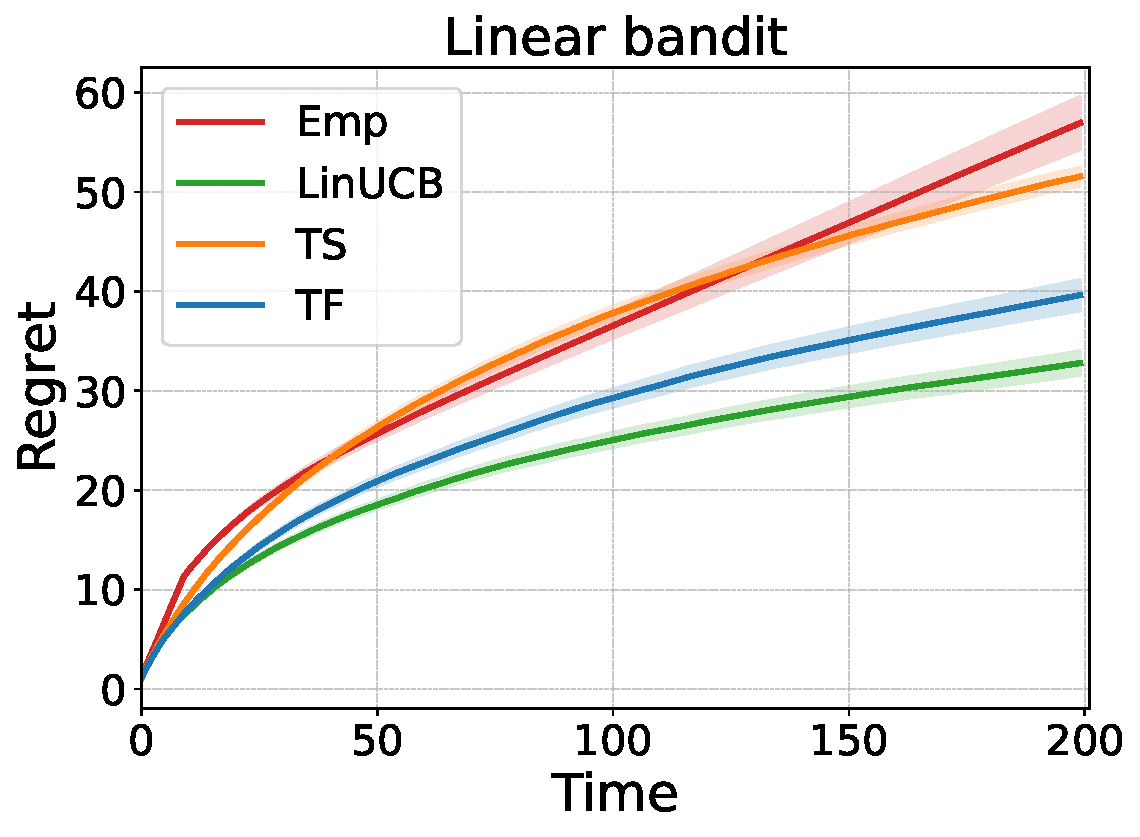
\includegraphics[width=0.35\linewidth]{Sections/figs/record_2_cum_True.pdf}
\hspace{2em}
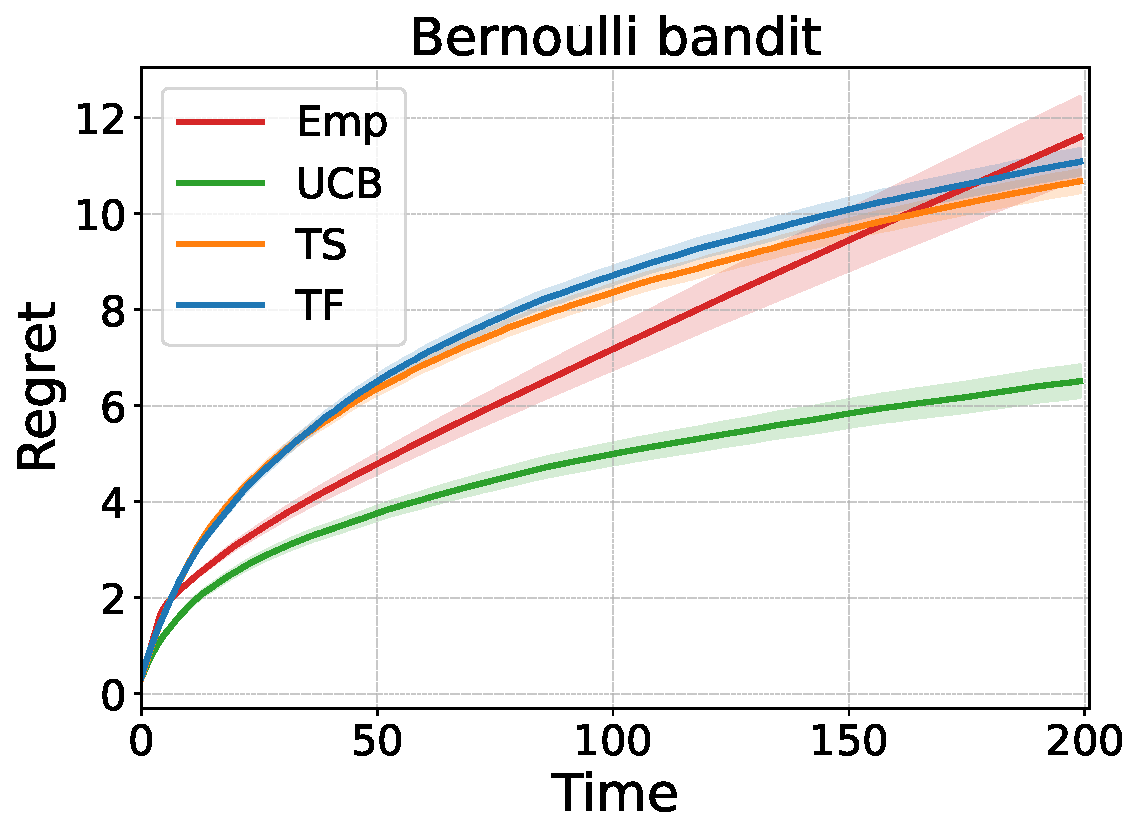
\includegraphics[width=0.35\linewidth]{Sections/figs/record_1_cum_True.pdf}
\vspace{-1em}
\caption{Regrets of transformer (TF), empirical average (Emp), Thompson sampling (TS) and LinUCB or UCB (LinUCB reduces to UCB for Bernoulli bandits). Left: linear bandit with $d=5$, $A=10$, $\sigma=1.5$, $\sAlg_0=\sAlg_\shortexp=\LinUCB$. Right: Bernoulli bandit with $d=5$, $\sAlg_0=(\sAlg_{\mathrm{unif}}+\sAlg_{\TS})/2$ and $\sAlg_\shortexp=\action^*$. The simulation is repeated 500 times. Shading displays the standard deviation of the regret estimates. }
\label{fig:regret_1}
\end{figure}


\section{Conclusions}

This paper theoretically investigates the ICRL capability of supervised-pretrained transformers. We demonstrate how transformers can efficiently implement prevalent RL algorithms including LinUCB, Thompson sampling, and UCB-VI, achieving near-optimal regrets in respective settings. We also provide sample complexity guarantees for the supervised pretraining approach to learning these algorithms. The generalization error scales with the covering number of the transformer class as well as the distribution ratio between the expert and offline algorithms. Simulations validate our theoretical findings.
Finally, we discuss the limitations of our results and provide additional discussions in Appendix~\ref{sec:limitation}.





\section*{Acknowledgement}

The authors would like to thank Peter L. Bartlett for the valuable discussions, and Jonathan Lee for the valuable discussions regarding Decision-Pretrained Transformers as well as providing an early version of its implementation. This work is supported by NSF CCF-2315725, DMS-2210827, NSF Career award DMS-2339904, and an Amazon Research Award.
\bibliography{references}
\bibliographystyle{plainnat}
\end{document}
